\chapter{Конструкторская часть}
В этом разделе будут приведены схемы алгоритмов и вычисления трудоемкости данных алгоритмов.
\section{Разработка алгоритмов}




На рисунках  \ref{fig:bubble}, \ref{fig:quick} и \ref{fig:comb} представлены схемы алгоритмов сортировки пузырьком, быстрой и расческой соответственно.

\begin{figure}[H]
	\centering
	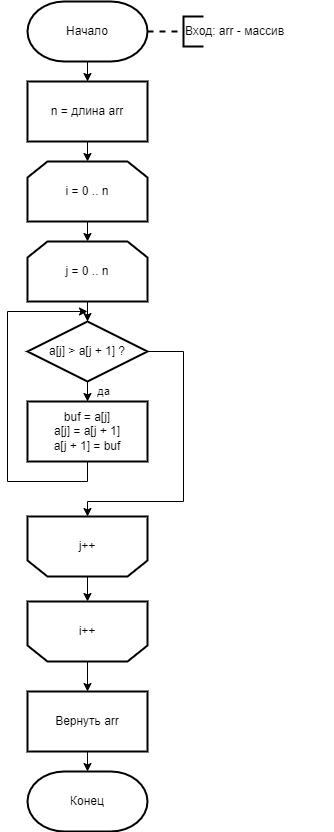
\includegraphics[width=0.7\linewidth, height=0.9\textheight]{inc/img/bubble}
	\caption{Схема алгоритма сортировки пузырьком}
	\label{fig:bubble}
\end{figure}

\begin{figure}[H]
	\centering
	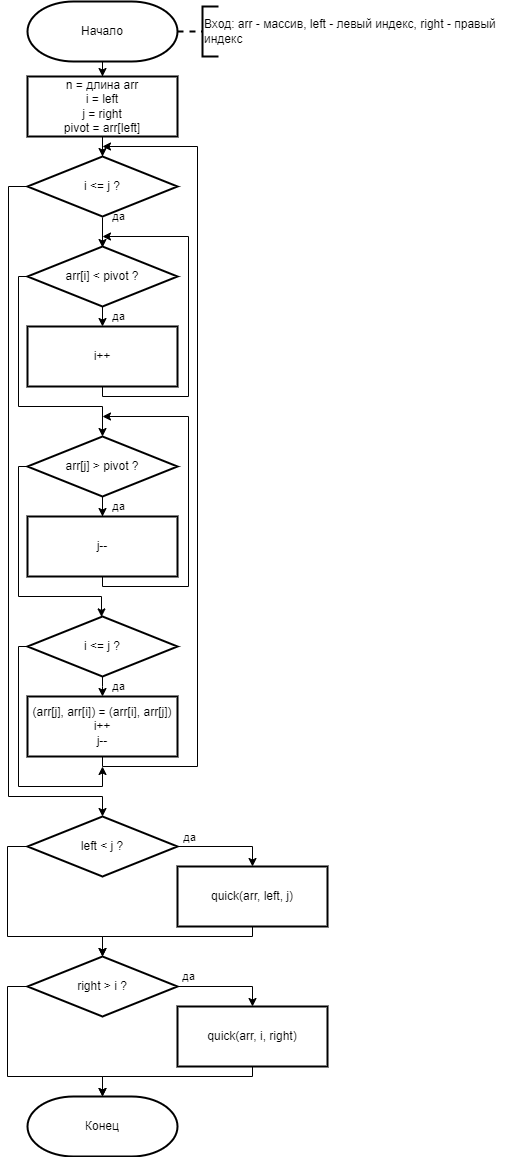
\includegraphics[width=0.7\linewidth, height=0.9\textheight]{inc/img/quick}
	\caption{Схема алгоритма быстрой сортировки}
	\label{fig:quick}
\end{figure}
\begin{figure}[H]
	\centering
	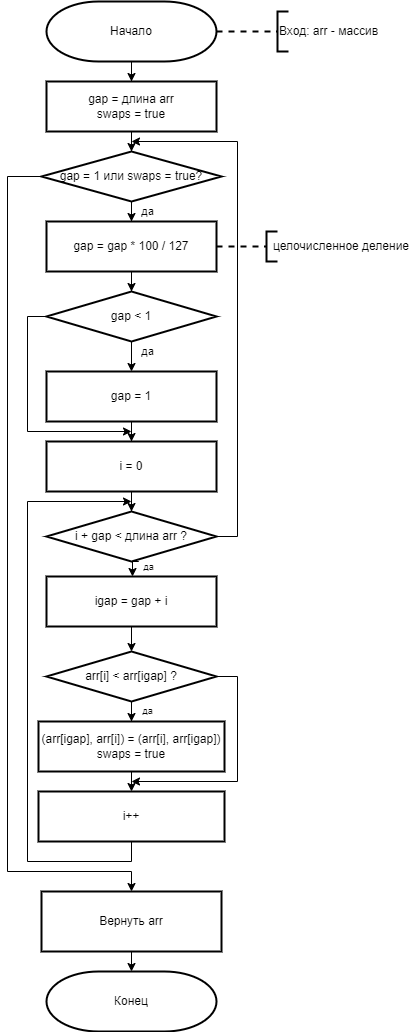
\includegraphics[width=0.7\linewidth, height=0.9\textheight]{inc/img/comb}
	\caption{Схема алгоритма сортировки расческой}
	\label{fig:comb}
\end{figure}

\section{Модель вычислений}

Для последующего вычисления трудоемкости необходимо ввести модель вычислений, или оценки трудоемкости.
\begin{enumerate}
	\item Операции из следующего списка имеют трудоемкость 1:
	\begin{equation}
		\label{for:opers}
		\begin{array}{cc}
		+, -, /, *, \%, =, +=, -=, *=, /=, \%=,\\
		==, !=, <, >, <=, >=, [], ++, {-}-
		\end{array}
	\end{equation}
	\item Трудоемкость оператора выбора \code{if условие then A else B} рассчитывается как
	\begin{equation}
		\label{for:if}
		f_{if} = f_{\text{условия}} +
		\begin{cases}
			f_A, & \text{если условие выполняется,}\\
			f_B, & \text{иначе.}
		\end{cases}
	\end{equation}
	\item Трудоемкость цикла рассчитывается как
	\begin{equation}
		\label{for:for}
		f_{for} = f_{\text{инициализации}} + f_{\text{сравнения}} + N(f_{\text{тела}} + f_{\text{инкремент}} + f_{\text{сравнения}})
	\end{equation}
	\item Трудоемкость вызова функции равна 0.
\end{enumerate}

\section{Трудоёмкость алгоритмов}

Обозначим во всех последующих вычислениях размер массивов как N.
\newpage
\subsection{Алгоритм сортировки пузырьком}

%fixed !! Тут должна быть вводная фраза перед формулой! Как и перед рисунком, таблицей, листингом. Добавлено вместе с недостающим f1

Трудоёмкость алгоритма сортировки пузырьком при прямом расчёте включает переменный член:

\begin{equation}
	f = 1 + 2 + (N - 1)(1 + 2 + 1 + 2 + \cancel{(N - i)}\cdot f{1},
\end{equation}
где $f{1}$ --- трудоёмкость сравнения элементов массива и тела условного оператора.

Количество выполненных сравнений известно:

\begin{equation}
Q_{\text{ср}} = \frac{a_{1} + a_{n}}{2} n = \frac{N^{2} - N}{2}
\end{equation}

На одно сравнение приходится следующая работа:

\begin{equation}
	f_{\text{ср}} = 4 + 
	\left[
		\begin{array}{ccc}
			0 \text{ лучший сл.}\\
			9 \text{ худший сл.}\\
		\end{array}
	\right.
	 + 1 + 2
\end{equation}
и 
\begin{equation}
f_{\text{служебные}} = 1 + 2 + (N - 1)(1 + 2 + 1 + 2)
\end{equation}
Итоговая трудоёмкость алгоритма сортировки пузырьком:

\begin{equation}
	f_{\text{п}} = N^{2} 
	\left[
		\begin{array}{ccc}
			7 / 2 \text{ лучший сл.}\\
			16 / 2 \text{ худший сл.}\\
		\end{array}
	\right.
	+ N
	\left[
		\begin{array}{ccc}
			6 - 7 / 2 \text{ лучший сл.}\\
			6 - 16 / 2 \text{ худший сл.}\\
		\end{array}
	\right.
	- 3
\end{equation}

При этом лучший случай достигается когда элементы в массиве расположены по возрастанию, а худший случай --- по убыванию. %....??, худший случай --- при  .... TODO

\subsection{Алгоритм быстрой сортировки}

Худший случай при несбалансированном дереве вызовов, т.е. количество вызовов равно количеству элементов массива. Таким образом временная сложность лучшего случая будет равна $O(N^{2})$.

Лучший случай при сбалансированном дереве вызовов, т.е. количество вызовов равно высоте дерева $\log(N)$. Таким образом временная сложность лучшего случая будет равна $O(N\log(N)$.


\subsection{Алгоритм сортировки расческой}

\textbf{Худший случай}

Худший случай для этой сортировки наступает тогда, когда все элементы уже отсортированы, но в обратном порядке. 
\begin{equation}\label{eq1}
	a_{i} = N - floor( 100 * gap_{i} / 127 )
\end{equation}

\begin{equation}\label{eq2}
	gap_{i} = gap_{i}-1 - floor( 100 * (gap_{i}-1) / 127 )
\end{equation}
Если выразить верхнюю границу  $a_{i}$ из уравнения (\ref{eq1}) и рекуррентного соотношения (\ref{eq2}), будет получено выражение, содержащее члены второй и первой степени $N$ с константой, дающей верхнюю границу $N^{2}$. Таким образом, временная сложность наихудшего случая равна $O(N^{2})$.

\textbf{Лучший случай}

Для лучшего случая все массива должен быть отсортирован. В этом случае цикл с $gap = 1$ пройдет всего один раз. 

\begin{equation}
	\begin{array}{cc}
	a_{N} = n \\
	a_{N - 1} = \frac{N}{1.27} \\
	a_{N - 2} = \frac{N}{1.27^{2}} \\ 
	. . . \\
	a_{N - i} = \frac{N}{1.27^{i}} \\
	\end{array}
\end{equation}

\begin{equation}
	S_{N} = a_{1} + a_{2} + ... + a_{N}
\end{equation}

\begin{equation}
	S_{N} =  \sum_{r=1}^N (\frac{1}{1.27^{r}})
\end{equation}

\begin{equation}
	H_{N, r} = \sum_{r=1}^{N}(\frac{1}{kr})
\end{equation}

Для $k \approx 1$ $H_{N,1} \in O(\log(N))$

Таким образом трудоемкость сортировки расческой получилась $O(N\log(N))$.

В худшем случае алгоритм будет работать, как обычный $"$пузырек$"$.

Асимптотическая трудоёмкость алгоритма сортировки расческой $O(N^{2})$ в худшем случае и $O(N\log(N))$ --- в лучшем \cite{combsort}.

\section*{Вывод}

Были разработаны схемы всех трех алгоритмов сортировки, а именно алгоритма сортировки пузырьком, быстрой сортировки и сортировки расческой. Для каждого из них были рассчитаны и оценены лучшие и худшие случаи.


